\section{شرح روش پیشنهادی مقالات}
{ 	
	در این بخش ابتدا مسئله تطبیق دامنه را به صورت ریاضی بیان می‌کنیم. سپس مشکلات و چالش‌هایی که در حل این مسئله وجود دارد را بیان خواهیم کرد. در ادامه نیز توضیح خواهیم داد که هر کدام از مقاله‌ها چه روشی را برای حل این مشکلات و چالش‌ها ارائه داده‌اند.
	
	\subsection{تعریف ریاضی مسئله تطبیق دامنه}
	{
		ما یک دامنه‌ی برچسب خورده به نام دامنه مبدا و یک دامنه برچسب نخورده به نام دامنه هدف داریم که به ترتیب به  صورت 
		$\left\{x_{s_i},\ y_{s_i}\right\}_{i=1} ^ n $
		و 
		$\left\{x_{t_j}\right\}_{j=1} ^ m$
		تعریف می‌شود. همچینین فرضیاتی را در مورد فضای ویژگی‌ها
		$X_s = X_t$
		و فضای برچسب‌ها
		$Y_s=Y_t$
		و احتمال حاشیه‌ای  
		${P_s(x}_s)\neq{P_t(x}_t)$
		و احتمال شرطی
		${P_s(y_s|x}_s)\neq{P_t(y_t|x}_t)$
		در نظر می‌گیریم. بنابراین هدف انتقال یادگیری این است که فضای برچسب‌های دامنه هدف 
		$Y_t$
		را به کمک دامنه مبدا
		$D_s$
		یاد بگیرد. تطبیق دامنه تلاش می‌کند که با کاهش واگرایی احتمال‌های حاشیه‌ای و احتمال‌های شرطی  بین دامنه‌ی مبدا و هدف، مسئله انتقال یاد گیری را حل کند به عبارت دیگر واگرایی بین 1)
		${P_s(x}_s)$
		و 
		${P_t(x}_t)$
		، 2) 
		${P_s(y_s|x}_s)$
		و
		${P_t(y_t|x}_t)$
		را به حداقل می‌رساند.
	}

	\subsection{تطبیق  متوازن توزیع در انتقال یادگیری
		\protect \footnote{\lr{Balanced Distribution Adaptation for Transfer Learning}}}
	{
		بسیاری از روش‌های تطبیق توزیع موجود، یکی از توزیع‌های حاشیه‌ای یا شرطی و یا هر دو را تطبیق می‌دهند. در مقاله‌های اخیر ثابت شده است که استفاده از هر دو توزیع عملکرد بهتری را نتیجه می‌دهد. اما روش‌های کنونی تاثیر هر دو توزیع را یکسان در نظر می‌گیرند در حالی که وقتی مجموعه‌داده‌ها بسیار متفاوت باشند، به این معنی است که توزیع حاشیه‌ای اهمیت بیشتری دارد و وقتی مجموعه‌داده‌ها مشابه هستند، به این معنی است که توزیع شرطی به توجه بیشتری نیاز دارد. از این رو، لازم است از هر دو توزیع با وزنی مناسب با اهمیت آن‌ها برای تطبیق استفاده نمود. علاوه بر این، نامتوازن بودن مجموعه‌داده بر روی تطبیق دامنه تاثیرگذار است که در روش‌های موجود، این موضوع در نظر گرفته نمی‌شود. برای حل این دو مشکل، در
		\cite{wang2017balanced}
		دو روش پیشنهاد شده است. روش اول BDA است که نه تنها می‌تواند توزیع‌های حاشیه‌ای و شرطی بین حوزه‌ها را تطبیق دهد، بلکه اهمیت این دو توزیع را به صورت متوازن تنظیم می‌کند. روش دوم
		\lr{W-BDA}
		است که مشکل نامتوازن بودن مجموعه‌داده را حل می‌کند.
		\lr{W-BDA}
		می‌تواند هنگام انجام تطبیق توزیع، وزن هر کلاس را به طور انطباقی تغییر دهد.
	 	\subsubsection{BDA}
	 	{
 		همانطور که توضیح دادیم در تطبیق دامنه، با کاهش واگرایی یا فاصله‌ی بین احتمال‌های حاشیه‌ای و شرطی می‌توانیم دامنه‌های مبدا و هدف را تطبیق دهیم. این موضوع را می‌توانیم به صورت عبارت زیر بیان کنیم:
 		\begin{equation}
 			Dist\left(D_{s,}D_t\right)\approx Dist{(P\ (x}_s),{P(x}_t))+Dist({P(y_s|x}_s),{P(y_t|x}_t))
 			\label{eq:1}
 		\end{equation}
 		روش BDA به عبارت 
 		\ref{eq:1}
 		 یک ضریب توازن به نام $\mu$ اضافه می‌کند که میزان اهمیت توزیع حاشیه‌ا‌ی و شرطی را در مسائل مختلف تنظیم و کنترل می‌کند. پس عبارت 
 		\ref{eq:1}
 		 تبدیل می‌شود به:
 		 \begin{equation}
 			Dist\left(D_{s,}D_t\right)\approx(1-\mu)Dist{(P\ (x}_s),{P(x}_t))+\mu Dist({P(y_s|x}_s),{P(y_t|x}_t))
 			\label{eq:2}
 		 \end{equation}
 		  برای حل عبارت 
 		  \ref{eq:2}
 		  از روش MMD 
 		  \footnote{\lr{Maximum Mean Discrepancy}}
 		  برای تخمین توزیع‌های حاشیه‌ای و توزیع‌های شرطی استفاده می‌کنیم. بنابراین خواهیم داشت:
 		  \begin{equation}
 		  	 D \left( D_{s,}D_{t} \right)  \approx  \left( 1- \mu  \right)  \bigg \|\frac{1}{n} \sum _{i=1}^{n}x_{s_{i}} - \frac{1}{m} \sum _{j=1}^{m}x_{t_{j}}\bigg \| _{H}^{2} + \mu \sum _{c=1}^{C} \bigg \Vert \frac{1}{n_{c}} \sum _{x_{s_{i}} \in  D_{s}^{ \left( c \right) }}^{n}x_{s_{i}} - \frac{1}{m_{c}} \sum _{x_{t_{j}} \in  D_{t}^{ \left( c \right) }}^{n}x_{t_{j}} \bigg \Vert _{H}^{2}
 		  	 \label{eq:3}
 		  \end{equation}
 		  
 		  در عبارت 
 		 \ref{eq:3}
 		  ترم اول فاصله‌ی توزیع‌های حاشیه‌ای بین دامنه‌ها را نشان می‌دهد و ترم دوم هم فاصله‌ی توزیع‌های شرطی بین دامنه‌ها را نمایش می‌دهد. با بهره‌گیری از تکنیک‌های ماتریس و جبر خطی عبارت 
 		 \ref{eq:3}
 		  را می‌توان به صورت زیر نوشت
 		  \footnote{لطفا برای مشاهده جزئیات بیشتر عبارت 4 به مقاله‌ی اصلی مراجعه نمایید.}
 		  :
 		  \begin{equation}
	 	  \begin{aligned}
		  min \quad tr \left( A^{T}X \left( \left( 1 - \mu \right) M_{0} + \mu \sum _{c=1\mathrm{ }}^{C}M_{c} \right) X^{T}A \right) + \lambda \Vert A \Vert_{F}^{2} \\
		  s.t. \quad A^{T}XHX^{T}A = I, \quad  0  \leq \mu \leq  1 \quad \quad \quad \quad \quad
		  \label{eq:4}
	 	  \end{aligned}
 		  \end{equation}
 		   در عبارت
 		   \ref{eq:4}
 		    دو ترم وجود دارد: 1) تطبیق توزیع‌های حاشیه‌ای و شرطی به همراه ضریب توازن $\mu$ 2) ترم مربوط به رگلاریسیون با ضریب رگلاریسیون $\lambda$. در این عبارت 2 قید هم داریم. قید اول بیان می‌کند که داده‌ی تغییر یافته خصوصیات داخلی اصل داده را حفظ می‌کند. قید دوم نیز بازه‌ی ضریب توازن را نشان می‌دهد.
 		    
 		    برای حل عبارت 
 		    \ref{eq:4}
 		    از ضرائب لاگرانژ استفاده می‌کنیم. بنابراین اگر ضرائب لاگرانژ 
 		    $\phi = \left\lbrace \phi_1, \phi_2, ... , \phi_d \right\rbrace  $
 		    باشد، خواهیم داشت: 
 		    \begin{equation}
 		    	\begin{aligned}
 		    	L = tr \left( A^{T}X \left( \left( 1 - \mu \right) M_{0} + \mu \sum _{c=1\mathrm{ }}^{C}M_{c} \right) X^{T}A \right) + \lambda \Vert A \Vert_{F}^{2} + tr \left( \left( I -  A^{T}XHX^{T}A)\right) \phi \right) 
 		    	\label{eq:5}
 		    	\end{aligned}
 		    \end{equation}
 		    
 		    برای بدست آوردن ماتریس تبدیل $A$ کافی است از عبارت
 		    \ref{eq:5}
 		    نسبت به $َA$ مشتق بگیریم و برابر صفر بگذاریم. در این صورت به عبارت زیر دست می‌یابیم:
 		    \begin{equation}
 		    	\left( X \left( \left( 1 - \mu \right) M_{0} + \mu \sum _{c=1\mathrm{ }}^{C}M_{c} \right) X^{T} + \lambda I \right) A = XHX^{T}A \phi
 		    	\label{eq:6}
 		    \end{equation}
 		 	عبارت 
 		 	\ref{eq:6}
 		 	همان معادله‌ی معروف بردار و مقدار ویژه است. پس با پیدا کردن d بردار ویژه با کمترین مقدار ویژه خواهیم توانست ماتریس تبدیل $A$ را بدست آوریم. در اینجا سوالی پیش می‌آید که چرا مقدار بهینه
 		 	$\mu$
 		 	 را بدست نیاوردیم. نکته‌ی حائز اهمیت در اینجا این است که پارامتر 
 		 	$\mu$
 		 	 یک پارامتر آزاد نیست که بتوانیم آن را تخمین بزنیم بلکه 
 		 	$\mu$
 		 	 با توجه به توزیع داده‌ها تخمین زده می‌شود. بنابراین در واقعیت باید با توجه به کاربرد و با استفاده از روش ارزیابی متقابل
 		 	 \footnote{\lr{Cross Validation}}
 		 	  مقدار بهینه 
 		 	$\mu$
 		 	 را بدست آوریم.
 		 	 \begin{figure}
 		 	 	\centering
 		 	 	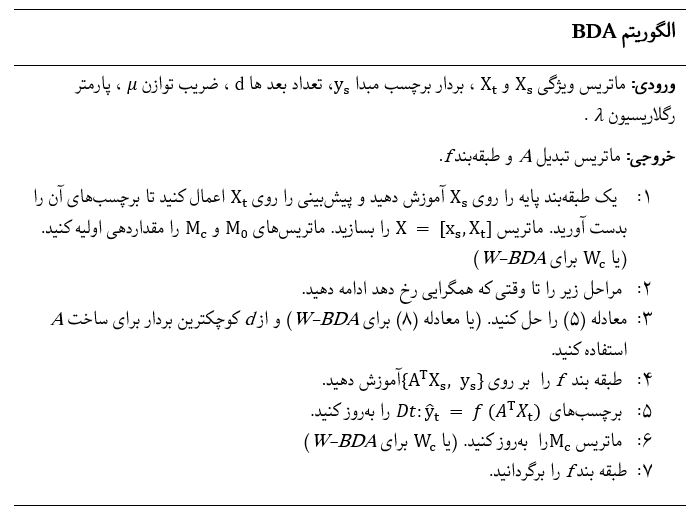
\includegraphics[scale=0.5]{images/table1.jpg}
 		 	 	\caption{}
 		 	 	\label{fig:5}
 		 	 \end{figure}
 		}
	 	\subsubsection{W-BDA}
	 	{
	 		روش 
	 		\lr{W-BDA}
	 		\footnote{\lr{Weighted Balanced Distribution Adaptation}}
	 		همانند روش 
	 		\lr{BDA}
	 		است با این تفاوت که با در نظر گرفتن نامتوازن بودن کلاس‌ها در داده‌ها تخمین دقیق‌تری را برای احتمال شرطی تعریف می‌کند.  همانطور که می‌دانیم در واقعیت ما نمی‌توانیم احتمال 
	 		$P(y|x)$
	 		را به صورت مستقیم تخمین بزنیم به همین دلیل با استفاده از قانون بیز به جای آن احتمال 
	 		$P(x|y)$
	 		را تخمین می‌زنیم. روش 
	 		\lr{W-BDA}
	 		برای تخمین احتمال پیشین داده‌های موجود در دامنه مبدا و هدف به ترتیب از دو ضریب 
	 		$\alpha_s$
	 		و 
	 		$\alpha_t$
	 	  استفاده می‌کند که با استفاده از آن‌ها تناسب کلاس‌های هر دامنه را متوازن می‌کند. اگر بخواهیم این مسئله را به صورت ریاضی بیان کنیم خواهیم داشت:
	 		\begin{equation}
	 		\begin{aligned}
	 		Dist({P(y_s|x}_s),{P(y_t|x}_t))= \Vert P \left( y_{s} \vert x_{s} \right)  -P \left( y_{t} \vert x_{t} \right) \Vert  _{H}^{2}\\
	 		= \bigg \Vert \frac{P \left( y_{s} \right) }{P \left( x_{s} \right) }P \left( y_{s} \vert x_{s} \right)  -\frac{P \left( y_{t} \right) }{P \left( x_{t} \right) }P \left( y_{t} \vert x_{t} \right) \bigg \Vert  _{H}^{2}\quad \quad \quad \quad \quad\\
	 		= \Vert \alpha _{s}P \left( y_{s} \vert x_{s} \right)  - \alpha _{t}P \left( y_{t} \vert x_{t} \right)  \Vert  _{H}^{2} \quad \quad \quad \quad \quad \quad \quad \quad \quad 
	 		\end{aligned}
	 		\label{eq:7}
	 		\end{equation}
	 		
	 		بنابراین با توجه به توضیحات بالا در روش 
	 		\lr{W-BDA}
	 		کافی است معادله‌ی 
	 		\ref{eq:4}
	 		را به معادله‌ی زیر تغییر دهیم
	 		\footnote{
	 			لطفا برای دیدن جزئیات ماتریس
	 			 $W_{c}$  
	 			 در معادله
	 			 \ref{eq:8}
	 			  به مقاله اصلی مراجعه نمایید. }
	 		:
	 		\begin{equation}
	 		\begin{aligned}
	 		min \quad tr \left( A^{T}X \left( \left( 1 - \mu \right) M_{0} + \mu \sum _{c=1\mathrm{ }}^{C}W_{c} \right) X^{T}A \right) + \lambda \Vert A \Vert_{F}^{2} \\
	 		s.t. \quad A^{T}XHX^{T}A = I, \quad  0  \leq \mu \leq  1 \quad \quad \quad \quad \quad
	 		\label{eq:8}
	 		\end{aligned}
	 		\end{equation}
	 		حل معادله‌ی 
	 		\ref{eq:8}
	 		مانند معادله‌ی 
	 		\ref{eq:4}
	 		است.
	 	
	 	به طور خلاصه الگوریتم دو روش 
	 	\lr{BDA}
	 	و
	 	\lr{W-BDA}
	 	را می‌توانید در شکل
	 	\ref{fig:5}
	 	 مشاهده کنید.
	 		
	 	}
	}

	\subsection{انتقال یادگیری آسان با استفاده از ساختارهای درون دامنه
		\protect \footnote{\lr{Easy Transfer Learning By Exploiting Intra-domain Structures}}}
	{
		\begin{figure}
			\centering
			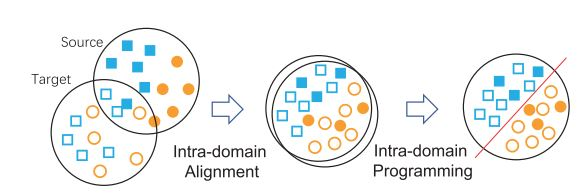
\includegraphics[scale=0.6]{images/easyTL.JPG}
			\caption{ فرآیند روش 
				\lr{\textit{EasyTL}}
				\cite{wang2019easy}.
			}
			\label{fig:6}
		\end{figure}
		بیشتر روش‌های سنتی و عمیق در انتقال یادگیری، روش‌های پارامتری است که باید طی فرآیندی بسیار گران قیمت و وقت گیر پارامترهای آن تنظیم شود. ارزیابی متقابل، که متداول‌ترین استراتژی برای انتخاب مدل‌ها و تنظیم پارامترها است، در انتقال یادگیری قابل استفاده نیست زیرا اغلب داده‌های برچسب خورده در دامنه هدف وجود ندارد. اگرچه روش‌های اخیر AutoML می‌تواند به طور خودکار پارامترها را از طریق هرس درخت و شبکه‌های عصبی تنظیم کنند اما آن‌ها قادر به مدیریت توزیع‌های مختلف بین دامنه‌ها نیستند و به طور معمول مدت زمان زیادی برای همگرایی لازم دارند. در 
		\cite{wang2019easy}
		الگوریتمی پیشنهاد شده است که روشی ساده اما کارآمد را پیشنهاد می‌دهد که علاوه بر این‌که مشکلات ذکر شده را حل می‌کند، این امکان را فراهم می‌کند که بتوان الگوریتم یادگیری انتقال را بر روی دستگاه‌های کوچک که دارای منایع محاسباتی محدود هستند نیز اجرا کرد. اسم این روش را
		\lr{\textit{EasyTL}}
		نامیدند.
		\lr{\textit{EasyTL}} 
		قادر است بدون نیاز به انتخاب مدل و تنظیم هایپرپارامترها ، انتقال دانش را در دامنه‌ها انجام دهد.
		\lr{\textit{EasyTL}}
		با بهره برداری از ساختارهای درون دامنه، هم انتقال ویژگی‌ها و هم انتقال طبقه‌بند را به صورت غیر پارامتری می‌آموزد. برای انتقال ویژگی‌ها روشی به نام
		\lr{\textit{intra-domain alignment}} 
		و برای انتقال طبقه‌بند روشی به نام
		\lr{\textit{intra-domain programming}} 
		را معرفی کرده است(شکل 
		\ref{fig:6}
		). در ادامه به توضیح جزئیات هر کدام از این روش‌ها می‌پردازیم.
		
		\subsubsection{\lr{intra-domain programming}}
		{
			در این بخش می‌خواهیم بررسی کنیم که روش 
			\lr{\textit{intra-domain programming}} 
			چگونه می‌تواند طبقه‌بند دامنه مبدا را به دامنه هدف منتقل کند. قبل از این‌که به جزئیات این روش بپردازیم، مفهومی را به نام ماتریس احتمال M معرفی می‌کنیم. سطر‌های این ماتریس تعداد کلاس‌ها و ستون‌های آن برابر با تعداد نمونه‌های موجود در مجموعه‌داده است. هر درایه از این ماتریس نشان می‌دهد که چقدر احتمال دارد یک نمونه متعلق به کلاس آن سطر باشد. بنابراین جمع احتمال‌های یک ستون در این ماتریس برابر یک است.
			\begin{figure}[h]
				\centering
				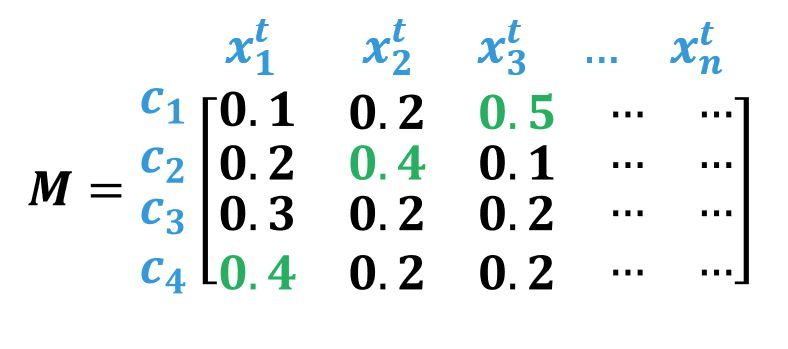
\includegraphics[scale=0.3]{images/annotation.JPG}
				\caption{یک مثال از ماتریس احتمال M .}
				\label{fig:7}
			\end{figure}
			(شکل
			\ref{fig:7})
			
			روش 
			\lr{\textit{intra-domain programming}} 
			به جای این‌که مستقیما 
			$y_t$
			را بیاموزد، تلاش می‌کند تا ماتریس احتمال M را بدست آورد. از این رو تابع هزینه به صورت زیر تعریف می‌شود:
			\begin{equation}
			\mathbf{J}=\ \sum_{j}^{n_t}\sum_{c}^{C}{D_{cj}}M_{cj}
			\label{eq:9}
			\end{equation}
			
			در عبارت 
			\ref{eq:9}
			ماتریس D ماتریس فاصله است که درایه‌ی 
			$D_{cj}$
			نشان‌دهنده‌ی فاصله‌ی نمونه
			$x_j^t$
			تا مرکز c‌ امین کلاس در دامنه مبدا است. اگر 
			$h_c$
			را به عنوان مرکز  c‌ امین کلاس در دامنه مبدا در نظر بگیریم؛ در این صورت 
			$D_{cj}$
			و 
			$h_c$
			به ترتیب به صورت زیر محاسبه می‌شود:
			\begin{equation}
			D_{cj}\ =\ \left|\left|x_t^j\ -\ h_c\right|\right|
			\label{eq:10}
			\end{equation}
			
			\begin{equation}
			h_c=\frac{1}{\left|\mathrm{\Omega}_s^{\left(c\right)}\right|}\sum_{i}^{n_s}{x_i^s.\ \mathbb{I}\left(y_i^s=c\right)}
			\label{eq:11}
			\end{equation}
			
			اکنون برای آن که ماتریس احتمال M را بدست آوریم باید تابع هزینه معادله
			\ref{eq:9}
			را به حداقل برسانیم. بدین منظور قیدهایی برای این تابع تعریف می‌شود. اولین قید این است که جمع احتمال هر ستون از ماتریس M برابر با یک باشد. قید دوم این است که حداقل باید برای هر کلاس یک نمونه وجود داشته باشد و قید سوم هم همانطور که می‌دانیم مقدار هر درایه از ماتریس M باید یک عدد در بازه‌ی صفر تا یک باشد. بنابراین به بیان ریاضی داریم:
			\begin{equation}
			\begin{aligned}
			min\ \ \ \ \mathbf{J}=\ \sum_{j}^{n_t}\sum_{c}^{C}{D_{cj}}M_{cj} \ \ \ s.t \\ 
			\sum_{c}^{C}M_{cj}=1,\ \forall\ j\ \epsilon\ 1,\ \ldots,\ n_t, \ \ \ \  \\ 
			\sum_{j}^{n_t}M_{cj}\geq1,\ \forall\ c\ \epsilon\ 1,\ \ldots,C,  \ \ \ \ \ \\ 
			0\le\ M_cj\le1\ \ \ \ \ \ \ \ \ \ \ \ \ \ \ \ \ \ \ \ \ \ \ \ \ \ \ \  \\
			\end{aligned}
			\label{eq:12}
			\end{equation}
			
			برای حل عبارت 
			\ref{eq:12}
			از کتابخانه PuLP در پایتون استفاده می‌کنیم و در نهایت ماتریس M بدست می‌آید. در گام آخر برچسب نمونه
			$x_j^t$
			به شکل زیر محاسبه می‌گردد:
			\begin{equation}
			y_{j}^{t}=\mathop{argmax}_{r}\frac{M_{rj}}{ \sum _{c}^{C}M_{cj}}\ \ \ \ \ \ for \ \ r \in  \{ 1,  \ldots , C \}
			\label{eq:13}
			\end{equation}
			
			نکته‌ی قابل توجه در این روش این است که هیچ پارامتری در این روش وجود ندارد که نیاز به تنظیم‌کردن داشته باشد. به همین علت است که این روش، یک روش غیر پارامتری است.
		}
		
		\subsubsection{\lr{intra-domain alignment}}
		{
			همان‌طور که در شکل 
			\ref{fig:6}
			مشخص است؛ هدف از 
			\lr{\textit{intra-domain alignment}}
			تطبیق ویژگی‌ها بین دامنه‌ی مبدا و هدف است که باعث کم شدن واگرایی بین دامنه‌ها می‌شود. روش‌های زیادی برای این کار وجود دارد مانند BDA‌ و GFK . اما در اینجا ما از روش 
			\lr{\textit{CORAL}}
			\footnote{\lr{CORrelation ALignment}}
			استفاده می‌کنیم که هم از لحاظ محاسباتی کارآمد است و هم یک روش غیرپارامتری است. فرمولی که این روش برای تطبیق دامنه‌ها معرفی می‌کند به صورت زیر است:
			\begin{equation}
				z^{r}= \bigg\{ \begin{array}{c}
				x^{r}.  \left( cov \left( x^{s} \right) +E_{s} \right) ^{-\frac{1}{2}}. \left( cov \left( x^{t} \right) +E_{t} \right) ^{\frac{1}{2}}\ \ \ \ \ if \ r=s\\
				x^{r} \ \ \ \ \ \ \ \ \ \ \ \ \ \ \ \ \ \ \ \ \ \ \ \ \ \ \ \ \ \ \ \ \ \ \ \ \ \ \ \ \ \ \ \ \ \ \ \ \ \ \ \ \ \ \ \ \ \ \ \ \ \ \ \   if \ r=t\\
				\end{array}
				\label{eq:14}
			\end{equation}
			
			\begin{figure}
				\centering
				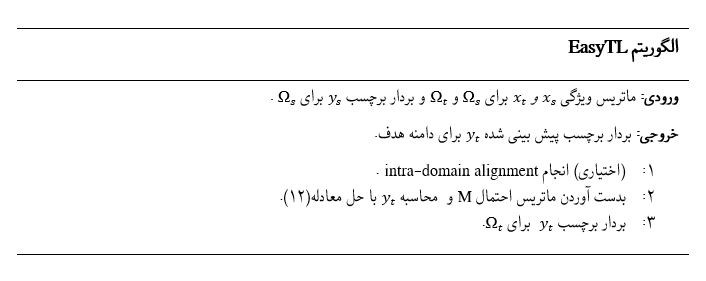
\includegraphics[scale=0.7]{images/easyTLAlgo.JPG}
				\caption{}
				\label{fig:8}
			\end{figure}
			
			الگوریتم روش 
			\lr{\textit{EasyTl}}
			را به طور خلاصه می‌توانید در شکل
			\ref{fig:8}
			مشاهده کنید.
		}
	}

}